\documentclass{article}
\usepackage[utf8]{inputenc}
\usepackage{amsmath}
\usepackage[a4paper,width=190mm,top=25mm,bottom=25mm,bindingoffset=2mm]{geometry}
\usepackage{graphicx} %package to manage images
\usepackage{subcaption} %package to manage sub-captions
\usepackage{float}
\usepackage{sectsty}
\usepackage{hyperref}
\sectionfont{\centering}
\bibliography{library}
\subsectionfont{\centering}
\usepackage{xcolor}
\graphicspath{ {./Images/} }
\usepackage[
backend=bibtex,
style=apa,
sorting=nyt,
uniquelist=true
]{biblatex}
\addbibresource{mybibliographyy.bib}

\title{Microlensing}
\author{Geet Purohit, Yoon Kyu Choi, Michael Polanco, George Kharchilava, and Aidan Boyce}
\date{November 2021}

\begin{document}
\begin{titlepage}
   \begin{center}
       \vspace*{1cm}
       \Huge {Paczynski Model Fitting for Gravitational Microlensing}
       \small
       \vspace{0.5cm}
       {\\Using the OGLE Microlensing 2019 Database}

       \vspace{1.5cm}
       \normalsize
       \textbf{Aidan Boyce, Yoon Kyu Choi, George Kharchilava, Michael Polanco, Geet Purohit}


       \vfill
       \Large
       Rutgers University\\
       November 2021
            
   \end{center}
\end{titlepage}

\section{Abstract}
Gravitational Microlensing events can be characterized by a few key parameters, which vary depending on the specific event being observed. Using these parameters, a light curve can be modeled against the observed data and such parameters can be extracted based on the data set given. In this report, the Paczynski Light Curve is used as the model for the data sets downloaded from the OGLE EWS (Optical Gravitational Lensing Experiment Early Warning System) website. Three complete data sets were chosen using a random number generator to minimize bias, each containing the magnitude measures, the time they were measured at, the magnitude errors, seeing estimation, and sky level. The parameters involved in the modelling are reported in the database as well. Those parameters are used to optimize the model estimates, by using a penalty function associated with the Paczynski Light Curve. Then, a Markov Chain Monte Carlo model fitting method is used to extrapolate the parameters from the fitted data. Using this method, the plots from the website can be replicated to test the reliability of this approach. The plots from this analysis match with those from the website, which is expected since the initial estimates are the reported parameter values from OGLE. 
%abstract

\section{Introduction}

Gravitational Microlensing occurs when a massive body (the lens) passes in front of a source of light from our perspective on Earth, causing a distortion in brightness for the duration of the event. These lens objects can vary from other massive stars, to point-mass objects. Such astrophysical phenomenons are detected and recorded by OGLE EWS (Optical Gravitational Lensing Experiment Early Warning System), and the information for this paper comes specifically from the OGLE-IV database. The Magnitude and Duration data from this research can be used to fit a Paczynski Light Curve Model, which will allow for the calculations of additional information about the event. In this paper, 3 sets of data will be used to provide a best-fit model of the Paczynski Light Curve, as well as the range of all possible parameter values for this model. This analysis will include the observed data of the events, the model fitting and its plots, analytical results of the model, and a discussion of the assumptions and limitations of the research. These assumptions will be critical in the analysis part of the paper and will be discussed further towards the end of it. 
% intro

\section{Methods}
\subsection{Data}

All of the data sets presented in this paper are from the OGLE-IV EWS database and were finalized in 2019, which is the most recent year of data since the operation had shut down due to the pandemic [\cite{OGLE}]. We used a random number generator to pick the data set numbers. We also made sure to include different types of data (messy vs clean) to produce unique results and analyze our models critically in all environments.

    \begin{figure}[h]
        \begin{subfigure}{0.329\textwidth}
            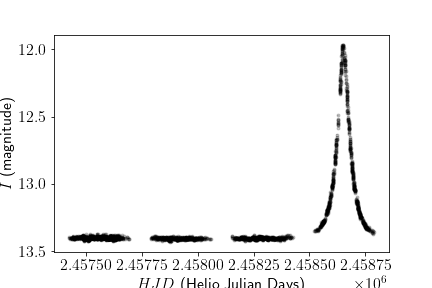
\includegraphics[width=1\linewidth, height=5cm]{Images/2019-BLG-148_Original_Data.png} 
            \caption{2019-BLG-0148}
            \label{fig:Mini-Event-One}
        \end{subfigure}
        \begin{subfigure}{0.329\textwidth}
            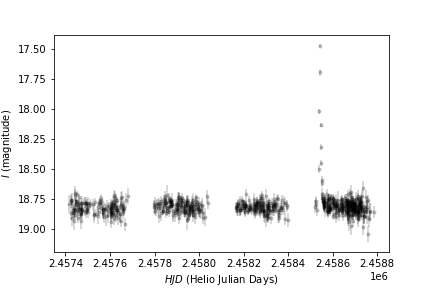
\includegraphics[width=1\linewidth, height=5cm]{Images/2019-BLG-0164_Original_Data.png}
            \caption{2019-BLG-0164}
            \label{fig:Mini-Event-Two}
        \end{subfigure}
        \begin{subfigure}{0.329\textwidth}
            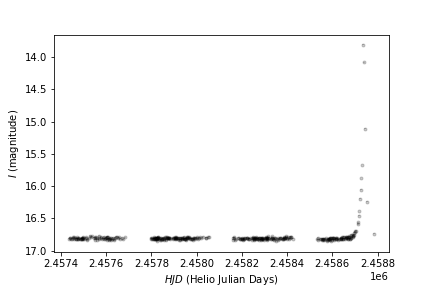
\includegraphics[width=1\linewidth, height=5cm]{Images/2019-BLG-1307_Original_Data.png}
            \caption{2019-BLG-1307}
            \label{fig:Mini-Event-Three}
        \end{subfigure}
    \caption{Three events chosen with a random number generator to minimize bias}
    \label{fig:image2}
    \end{figure}
    

\vspace{0.5cm}
\subsection{Model}
A derivation for the model begins with the known relations between  flux, magnitude, and luminosity:
$$
F=\frac{L}{4 \pi D^{2}}
$$
$$
m_{2}-m_{1}=2.5 \log _{10}\left(\frac{F_{1}}{F_{2}}\right) \\
$$


Substituting $F$ into Equation $2$ gives us:
$$
m_{2}-m_{1}=2.5 \log _{10}\left(\frac{L_{1}}{4 \pi D_{1}^{2}} \frac{4 \pi D_{2}^{2}}{L_{2}}\right) \\
$$

Another useful property of lensing is that it conserves surface brightness [\cite{keeton}]:

$$
\frac{f_{img}}{f_{src}} = \frac{dA_{img}}{dA_{src}} = |det\text{A}| = \texttt{Amplification of the image}
$$

Combining both of them, we get the model for a microlensing light curve (The Paczynski Light Curve). It describes the simplest approximation of a microlensing event, which is that both the lens and the source of light are considered point-like due to the vast distances from them to us [\cite{1996}]. It has the form:

$$
m(t) = m_{src} - 2.5 \text{log}_{10} [f_{bl} \cdot A(t) + (1 - f_{bl})]
$$
Where $m(t)$ is the apparent magnitude as a function of time, $m_{src}$ is the baseline magnitude, $f_{bl}$ is the blend parameter (which tells us what fraction of the $m_{src}$ comes from stars other than the source and other cosmic material), and $A(t)$ is the lensing amplification as a function of time. The lensing amplification $A(t)$ is also dependent on $u(t)$ as follows:
$$
\hspace{30pt} A(t) = \frac{u(t)^2 + 2}{u(t)\sqrt{u(t)^2 + 4}} \hspace{20pt} where \hspace{20pt} u(t) = \left[{u^2_{min}} + \left(\frac{t-t_{0}}{t_{E}}\right)^2\right]^\frac{1}{2}
$$
Here $u(t)$ is the angular separation of the lens and the source as a function of time, $u_{min}$ is the impact parameter (also known as the minimum distance), $t_{0}$ is the time when the light curve reaches its peak, and $t_{E}$ is the Einstein time scale for the event. Some models and research papers use ${\tau}$ and $t_{E}$ interchangeably. We used the $\chi^2$ penalty function :
$$
  \chi^2 = \sum_{i=1}^{N} \frac{ (f(x_i) - y_i )^2}{\sigma_i^2}
$$
For the Markov Chain Monte Carlo analysis, we defined a likelihood function $e^{\frac{\chi^2}{2}}$, so that $ln(L) = \frac{-\chi^2}{2}$ using emcee documentation [\cite{emceedocumentation}]. We also defined a prior function that constrained $f_{bl}$ to between 0 and 1. This is important because the prior function uses any prior knowledge we have about the parameter and uses it to draw samples from a probability distribution for the 5 parameters. We then used 20 walkers with 400 burn in steps and $\sim$2000 main run steps to extrapolate the 5 parameters from the fitted data.


\section{Results}
\subsection{Main Analysis}
Here we analyze the three data sets, BLG-0148, BLG-0164, and BLG-1307. We optimize values using \texttt{scipy.optimize.fmin}, where our initial guesses were the values published on the OGLE website.
\subsubsection{Data 1 : 2019-BLG-0148}
        \begin{figure}[H]
            \begin{subfigure}{0.5\textwidth}
                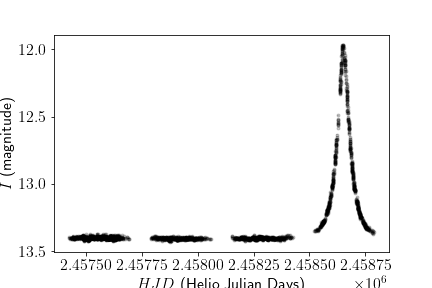
\includegraphics[width=1\linewidth, height=7cm]{Images/2019-BLG-148_Original_Data.png} 
                \caption{Data Set}
                \label{fig:Sub-Event-One-Main}
            \end{subfigure}
            \begin{subfigure}{0.5\textwidth}
                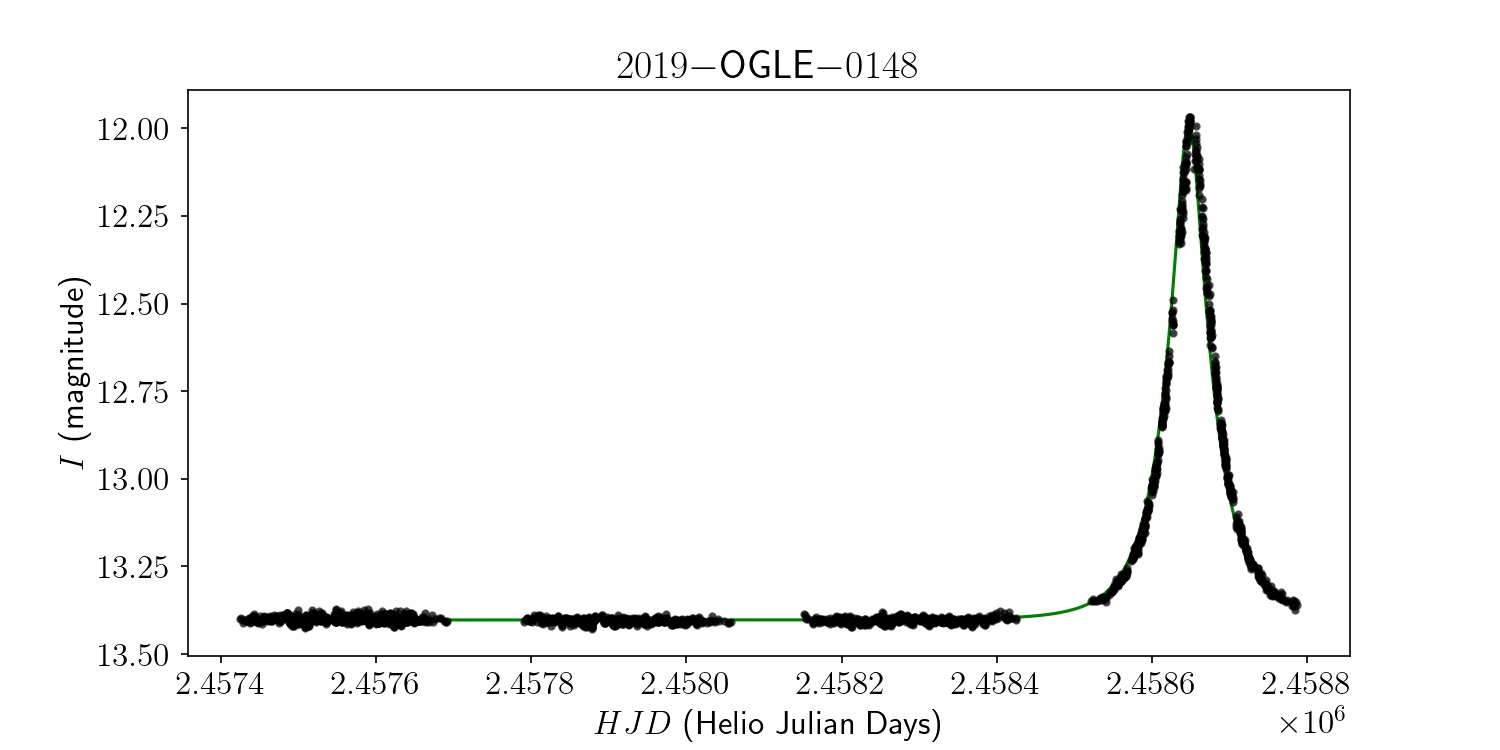
\includegraphics[width=1\linewidth, height=7cm]{Images/2019-BLG-0148_Original_Data_Model_fitted.png}
                \caption{Fitted Model}
                \label{fig:Sub-Event-One-Alt}
            \end{subfigure}
        \caption{2019-BLG-0148 data with the main data (left) and the model fitting (right)}
        \label{fig:image2}
        \end{figure}
    
        \begin{figure}[H]
            \begin{center}
                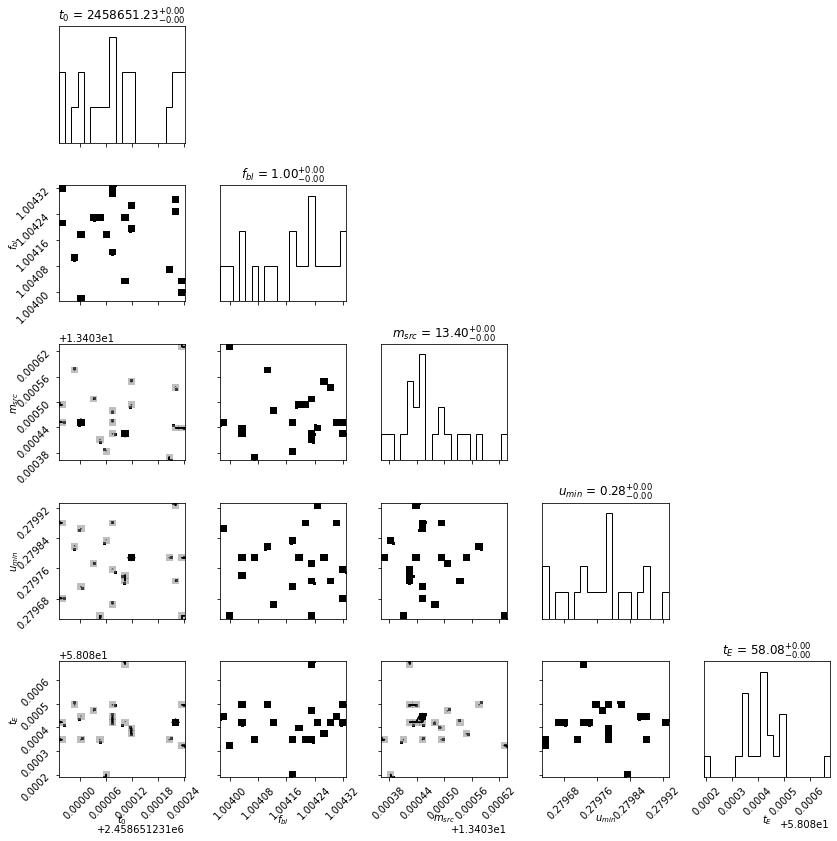
\includegraphics[scale = 0.35]{Images/2019-BLG-148_Corner_Plot.png}
                \caption{Corner Plot}
                \label{fig:2019-BLG-0001 Corner Plot}
            \end{center}
        \end{figure}
    
        \begin{table}[H]
            \renewcommand{\arraystretch}{1.5}
            \centering
            \caption{2019-BLG-0148 Parameter Values}
            \begin{tabular}{|c|c|c|c|c|c|}
                \hline
                \multicolumn{6}{|c|}{Parameters and Uncertainties}\\
                \hline
                Parameter: & $t_{0} (HJD)$ & $f_{bl}$ & $m_{src}$ & $u_{min}$ & $t_{E}$ \\
                \hline
                OGLE Published: & $2458651.232_{-0.007}^{+0.007}$ & $1.000_{-0.00}^{+0.00}$ & $13.403_{-0.00}^{+0.00}$ & $0.279_{-0.00}^{+0.00}$ & $58.205_{-0.0016}^{+0.0016}$\\
                \hline
                Best Model(Optimized Values): & $2458651.231$ & $1.00425$ & $13.4035$ & $0.2798$ & $58.08$\\
                \hline
                MCMC Median Values: & $2458651.23_{-0.00}^{+0.00}$ & $1.00_{-0.00}^{+0.00}$ & $13.40_{-0.00}^{+0.00}$ & $0.28_{-0.00}^{+0.00}$ & $58.08_{-0.00}^{+0.00}$\\
                \hline
            \end{tabular}
            \label{tab:2019-BLG-0001 Parameters}
        \end{table}
\vspace{1.5cm}     
\subsubsection{Data 2 : 2019-BLG-0164}
        \begin{figure}[H]
            \begin{subfigure}{0.5\textwidth}
                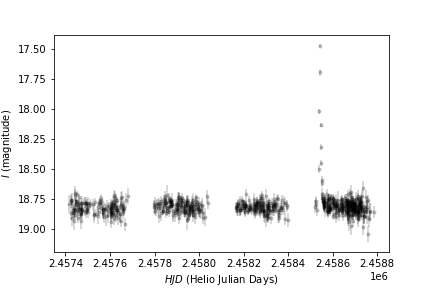
\includegraphics[width=1\linewidth, height=7cm]{Images/2019-BLG-0164_Original_Data.png} 
                \caption{Data Set}
                \label{fig:Sub-Event-One-Main}
            \end{subfigure}
            \begin{subfigure}{0.5\textwidth}
                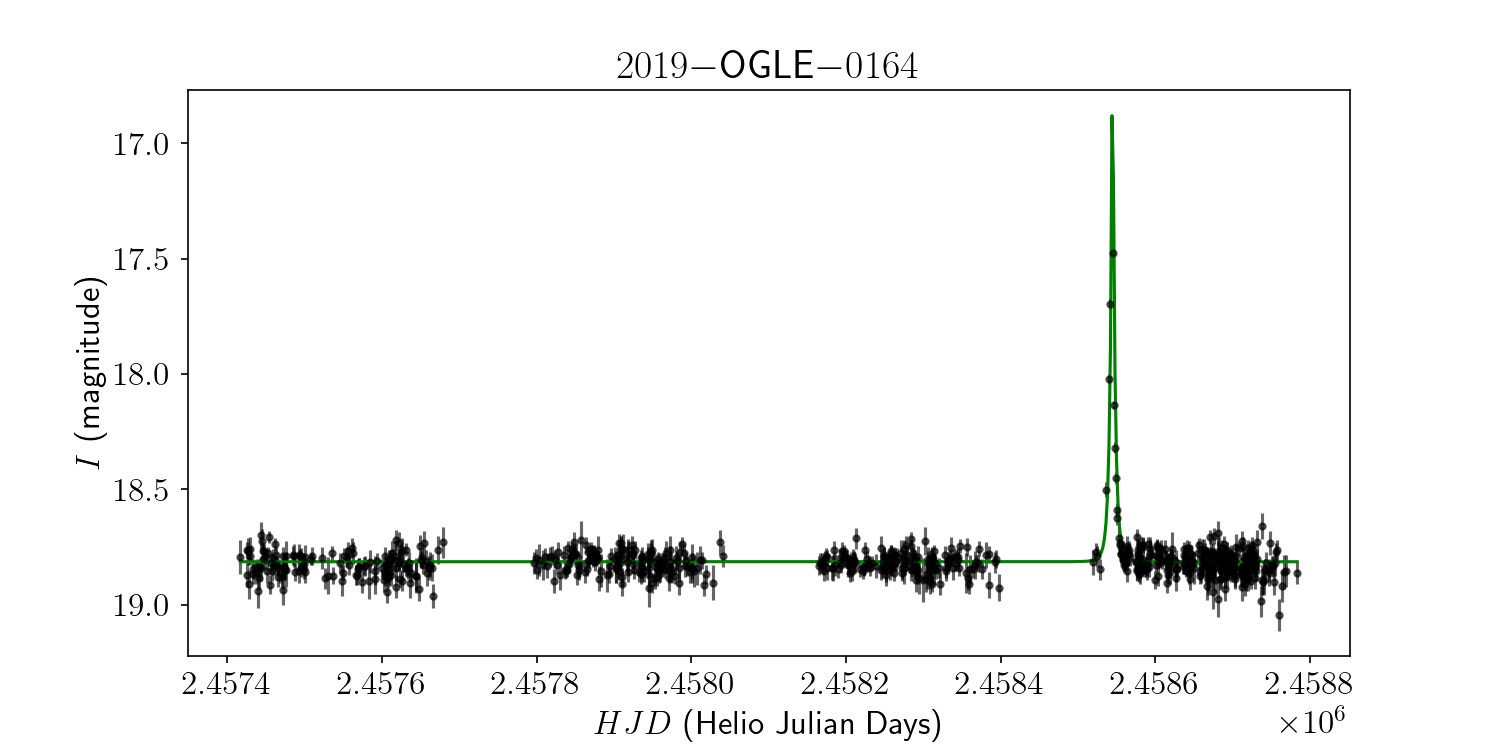
\includegraphics[width=1\linewidth, height=7cm]{Images/2019-BLG-0164_Original_Data_Model_fitted.png}
                \caption{Fitted Model}
                \label{fig:Sub-Event-One-Alt}
            \end{subfigure}
        \caption{2019-BLG-0164 data with the main data (left) and the model fitting (right)}
        \label{fig:image2}
        \end{figure}
    
        \begin{figure}[H]
            \begin{center}
                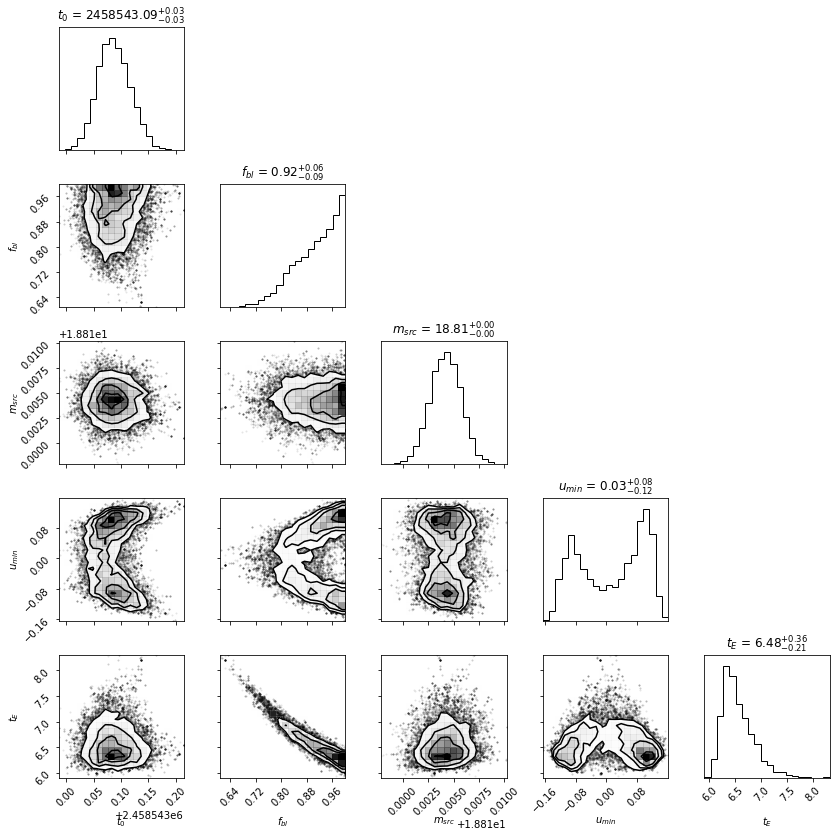
\includegraphics[scale = 0.35]{Images/2019-BLG-0164_Corner_Plot.png}
                \caption{Corner Plot}
                \label{fig:2019-BLG-0001 Corner Plot}
            \end{center}
        \end{figure}
    
        \begin{table}[H]
            \renewcommand{\arraystretch}{1.5}
            \centering
            \caption{2019-BLG-0164 Parameter Values}
            \begin{tabular}{|c|c|c|c|c|c|}
                \hline
                \multicolumn{6}{|c|}{Parameters and Uncertainties}\\
                \hline
                Parameter: & $t_{0} (HJD)$ & $f_{bl}$ & $m_{src}$ & $u_{min}$ & $t_{E}$ \\
                \hline
                OGLE Published: & $2458543.099_{-0.032}^{+0.032}$ & $1.000_{-0.00}^{+0.00}$ & $18.814_{-0.002}^{+0.002}$ & $0.118_{-0.019}^{+0.019}$ & $6.236_{-0.099}^{+0.099}$\\
                \hline
                Best Model(Optimized Values): & $2458543.11$ & $1.00$ & $18.814$ & $0.1239$ & $6.236$\\
                \hline
                MCMC Median Values: & $2458543.09_{-0.03}^{+0.03}$ & $0.92_{-0.09}^{+0.06}$ & $18.81_{-0.00}^{+0.00}$ & $0.03_{-0.12}^{+0.08}$ & $6.48_{-0.21}^{+0.36}$\\
                \hline
            \end{tabular}
            \label{tab:2019-BLG-0001 Parameters}
        \end{table}
        
\subsubsection{Data 3 : 2019-BLG-1307}
        \begin{figure}[H]
            \begin{subfigure}{0.5\textwidth}
                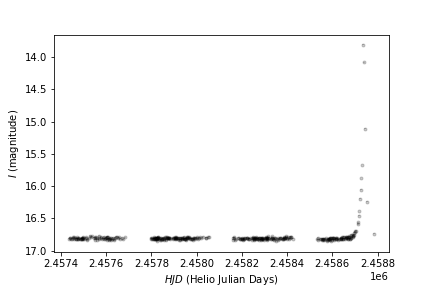
\includegraphics[width=1\linewidth, height=7cm]{Images/2019-BLG-1307_Original_Data.png} 
                \caption{Data Set}
                \label{fig:Sub-Event-One-Main}
            \end{subfigure}
            \begin{subfigure}{0.5\textwidth}
                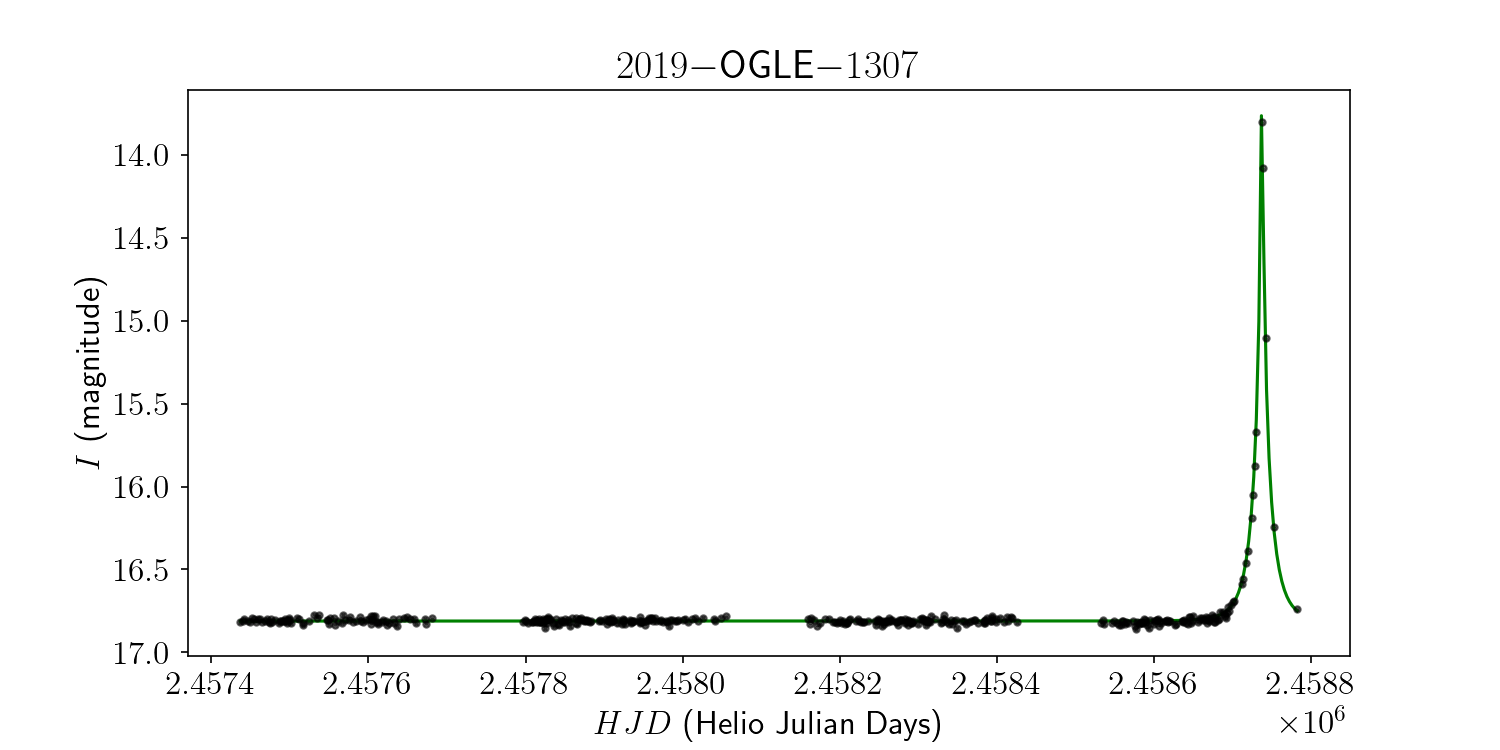
\includegraphics[width=1\linewidth, height=7cm]{Images/2019-BLG-1307_Original_Data_Model_fitted.png}
                \caption{Fitted Model}
                \label{fig:Sub-Event-One-Alt}
            \end{subfigure}
        \caption{2019-BLG-1307 data with the main data (left) and the model fitting (right)}
        \label{fig:image2}
        \end{figure}
    
        \begin{figure}[H]
            \begin{center}
                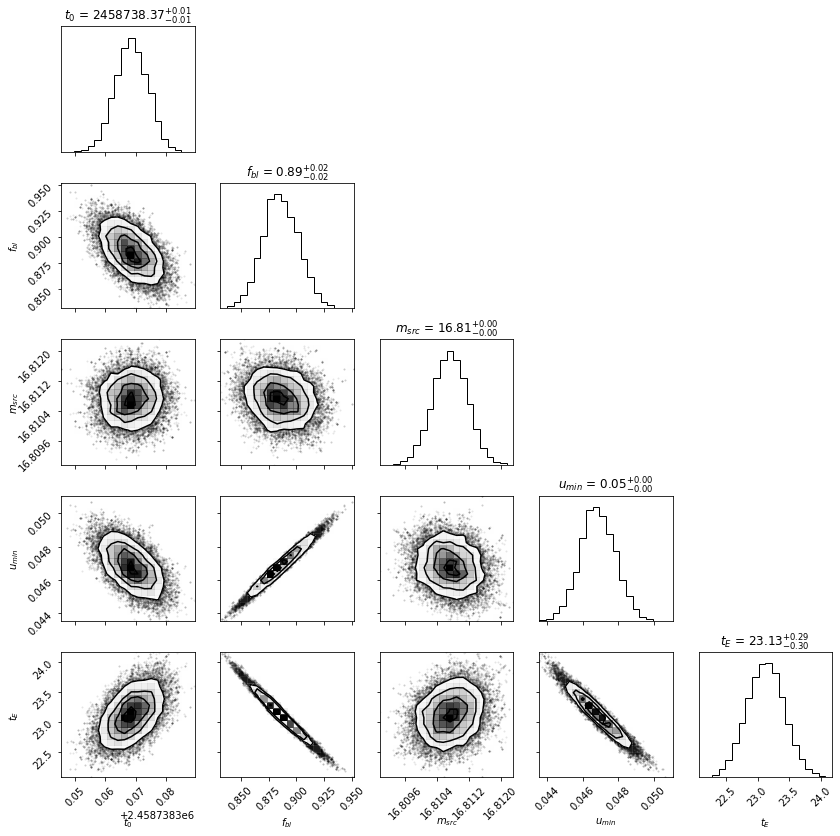
\includegraphics[scale = 0.35]{Images/2019-BLG-1307_Corner_Plot.png}
                \caption{Corner Plot}
                \label{fig:2019-BLG-0001 Corner Plot}
            \end{center}
        \end{figure}
    
        \begin{table}[H]
            \renewcommand{\arraystretch}{1.5}
            \centering
            \caption{2019-BLG-1307 Parameter Values}
            \begin{tabular}{|c|c|c|c|c|c|}
                \hline
                \multicolumn{6}{|c|}{Parameters and Uncertainties}\\
                \hline
                Parameter: & $t_{0} (HJD)$ & $f_{bl}$ & $m_{src}$ & $u_{min}$ & $t_{E}$ \\
                \hline
                OGLE Published: & $2458738.369_{-0.005}^{+0.005}$ & $0.885_{-0.016}^{+0.016}$ & $16.943_{-0.020}^{+0.020}$ & $0.047_{-0.001}^{+0.001}$ & $23.127_{-0.288}^{+0.288}$\\
                \hline
                Best Model(Optimized Values): & $2458738.371$ & $0.87311$ & $16.811$ & $0.046$ & $23.3615$\\
                \hline
                MCMC Median Values: & $245738.37_{-0.01}^{+0.01}$ & $0.89_{-0.02}^{+0.02}$ & $16.81_{-0.00}^{+0.00}$ & $0.05_{-0.00}^{+0.00}$ & $23.13_{-0.30}^{+0.29}$\\
                \hline
            \end{tabular}
            \label{tab:2019-BLG-0001 Parameters}
        \end{table}
\vspace{0.5cm}            
The optimized values and the median values from the MCMC analysis are very close to published OGLE values. Notably in Data set 1 (2019-BLG-0148), where the data points fit the model with a very high degree of accuracy. We see that there is almost no difference between the values in that case. We can delve deeper into the analysis of the variability by looking into the residuals of each analysis.

\vspace{0.5cm}    

\subsection{Residual Analysis}
When the model is fit to the data, we see that there isn't a big difference between the distribution of parameter values from the MCMC analysis and the published values from the OGLE website. However, there is a clear difference between data sets that are cleaner versus those that are not. The comparison between BLG-0148 and BLG-0164 shows that there is a better fit to the model for BLG-0148. This observation can be visualized using a residual analysis. This method includes taking the difference between the model y-values and the y values of the data points. Note that the y-values are the magnitudes, and the difference $\Delta y$ is the error value. Here is a comparison of the residual plots of BLG-0148 and BLG-0164:

        \begin{figure}[H]
            \begin{subfigure}{0.5\textwidth}
                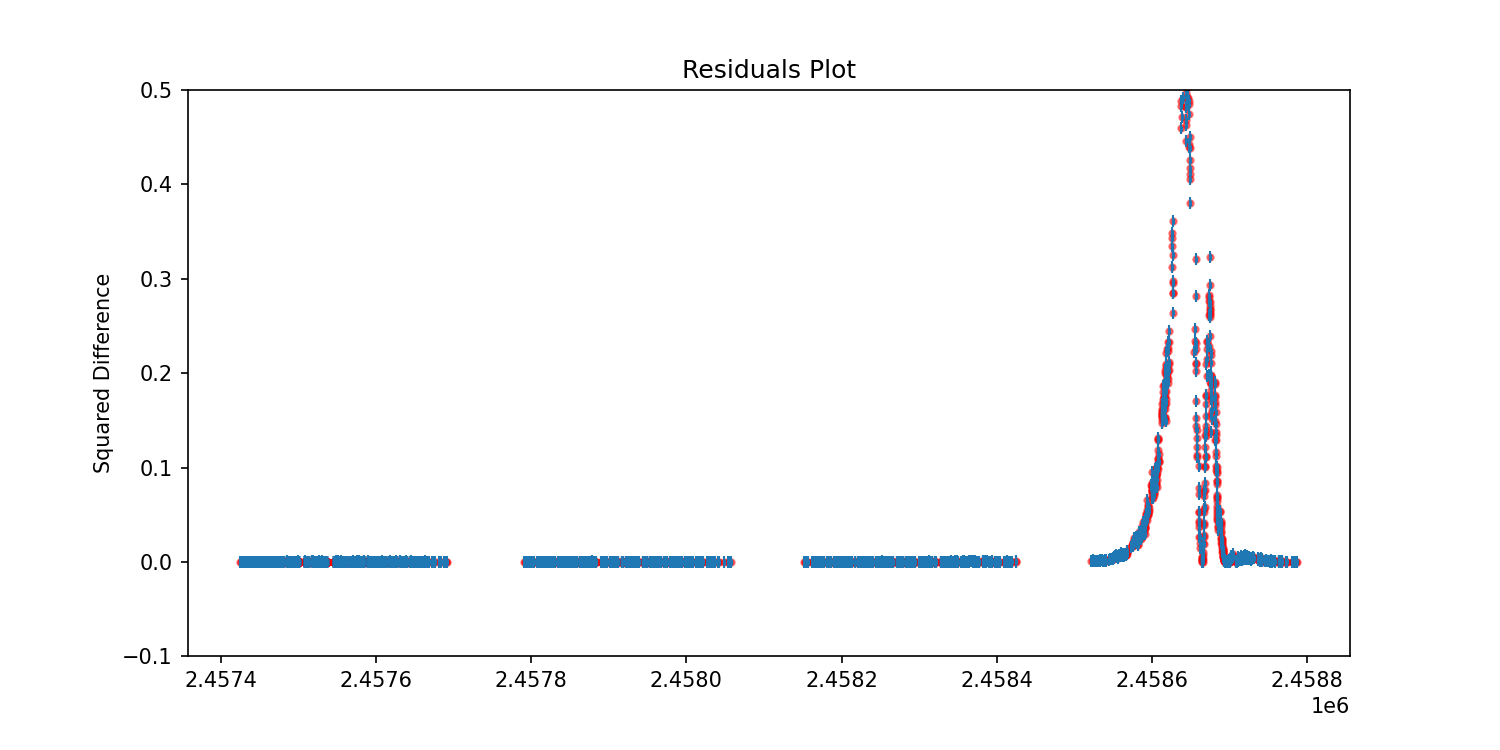
\includegraphics[width=1\linewidth, height=7cm]{Images/2019-BLG-0148_Residuals.png} 
                \caption{BLG-0148}
                \label{fig:Sub-Event-One-Main}
            \end{subfigure}
            \begin{subfigure}{0.5\textwidth}
                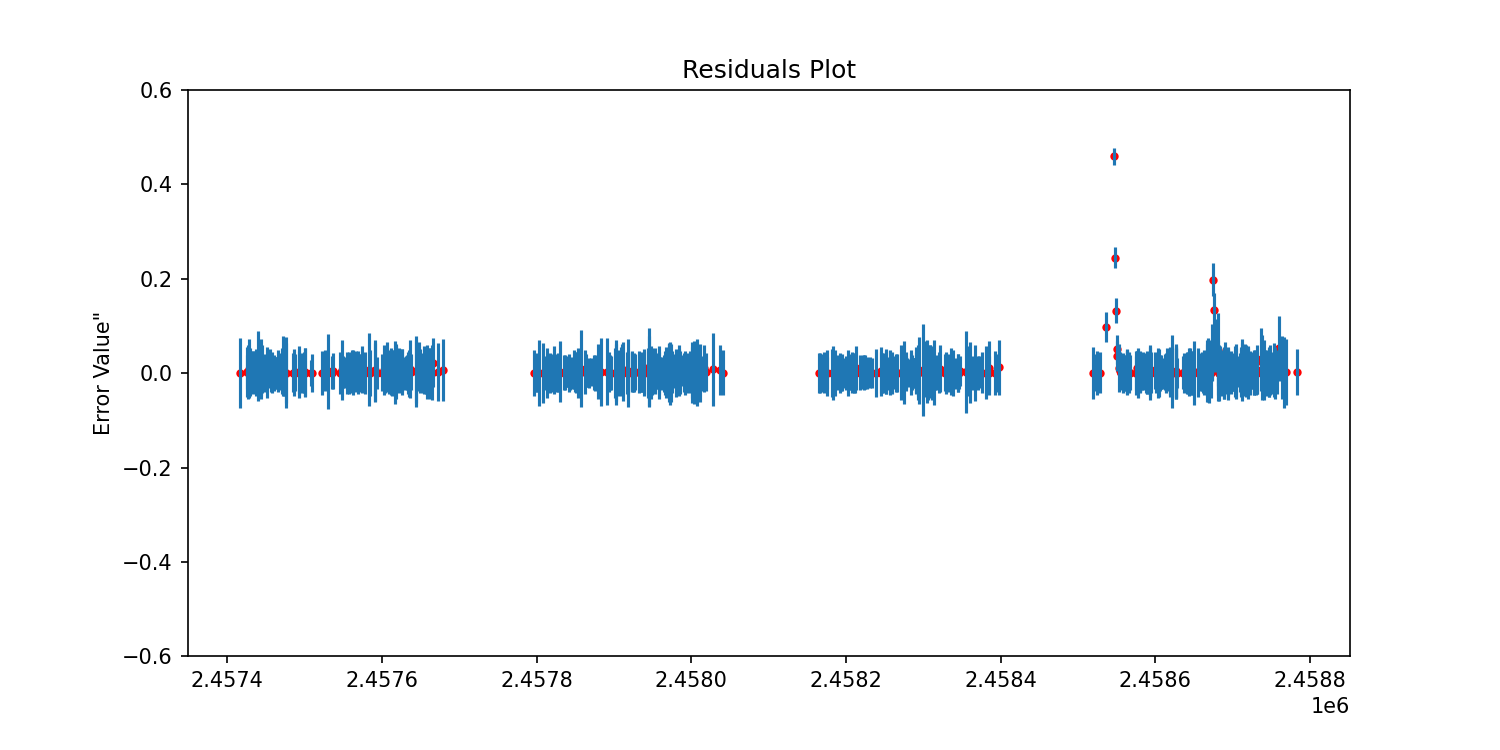
\includegraphics[width=1\linewidth, height=7cm]{Images/2019-BLG-0164_Residuals.png}
                \caption{BLG-0164}
                \label{fig:Sub-Event-One-Alt}
            \end{subfigure}
        \caption{Residual variability between clean distribution and messy distribution}
        \label{fig:image2}
        \end{figure}
        
The red dots in the graph are the actual data points corresponding to the squared differences, whereas the blue markers (in this case we used the pipe \texttt{|} character to denote it) are error denotation symbols. We can clearly see that the residual errors for the BLG-0164 are more consistent throughout the time scale of the event, while BLG-0148 maintains a clean pattern and minimal errors when a model is fit to the data. The range of these values for any general data set under observation is subject to the positional variability of the light source and the quality/handling of the recording instruments.

\section{Discussion}
\subsection{Bias Analysis}

The measurement of observed values from any Microlensing events is non-trivial unless certain assumptions are put in place. One of these fundamental assumptions is assuming that both the lensing and source objects act as points. Despite these objects being spherical, their large distances make this limitation negligible enough where the model can still accurately pass through the vast majority of the data points. As a result, there is no correction made to bypass this limitation

Another limitation that needs to be addressed is blend. This occurs when either the lensing objects or any objects between the source and the instrument contributes to the magnitude measured. An extra parameter $f_{bl}$, was added towards the late stages of this investigation after realizing that the effects of blend are not negligible [\cite{Wyrzykowski}]. When performing the optimization, the best-fit parameters were far off enough to transition the light curve off of the data points. In particular, it affected the predicted source magnitude the most, causing a simple shift in the line. The resulting chi-squared value was also large, far from the expected values (by multiple factors of 10), which can be inferred from the amount of data taken. A general trend was that after implementing the blend parameter, the $\chi^2$ values decreased and the parameters outputted were reasonable.  


\subsection{Data Quantification Analysis}
The data sets for model fitting were chosen with a random number generator to minimize bias. Additionally within the three data sets, one of them have a varied vertical distribution of data points. The first and the third data sets are very clean and provide a much better model fitting. This can be seen when the walkers in the burn-in run of the MCMC analysis don't oscillate between a range. A quick look at the walkers for the messy data versus clean data shows us the difference between the probability distribution of the parameters:

        \begin{figure}[H]
            \begin{subfigure}{0.5\textwidth}
                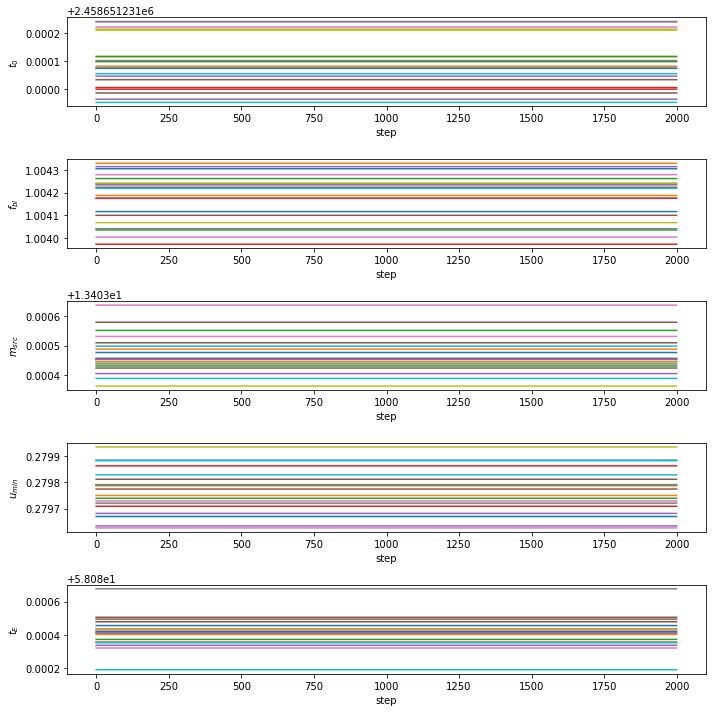
\includegraphics[width=1\linewidth, height=7cm]{Images/2019-BLG-148_Walkers_Plot.png} 
                \caption{BLG-0148}
                \label{fig:Sub-Event-One-Main}
            \end{subfigure}
            \begin{subfigure}{0.5\textwidth}
                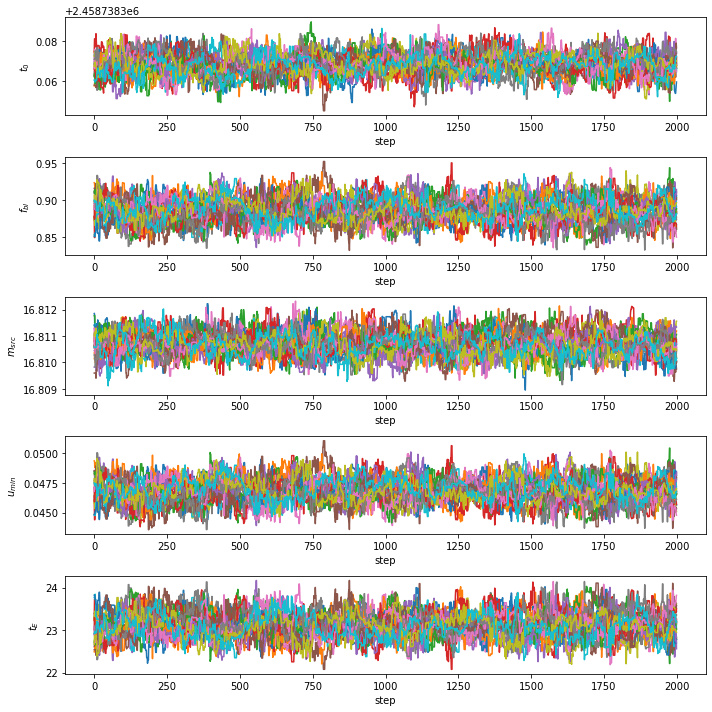
\includegraphics[width=1\linewidth, height=7cm]{Images/2019-BLG-1307_Walkers_Plot.png}
                \caption{BLG-1307}
                \label{fig:Sub-Event-One-Alt}
            \end{subfigure}
        \caption{Parameter variability between clean distribution and messy distribution}
        \label{fig:image2}
        \end{figure}
        
\subsection{Alternative Model Analysis}
It is worth mentioning that there are several different ways to obtain reasonable parameters. Optimization gives the best fit model to the data since it relies on minimizing a $\chi^2$ function. There are also the median values taken from the MCMC analysis (both upper and lower when errors are taken into account). Finally there is the average of all MCMC values for each parameter. To check the variability of these different parameter values, all five models were plotted together on the same plot for the BLG-0164 data set. We choose only this data set as it is the messiest, which implies that we expect to see the biggest residual differences here:
        \begin{figure}[H]
            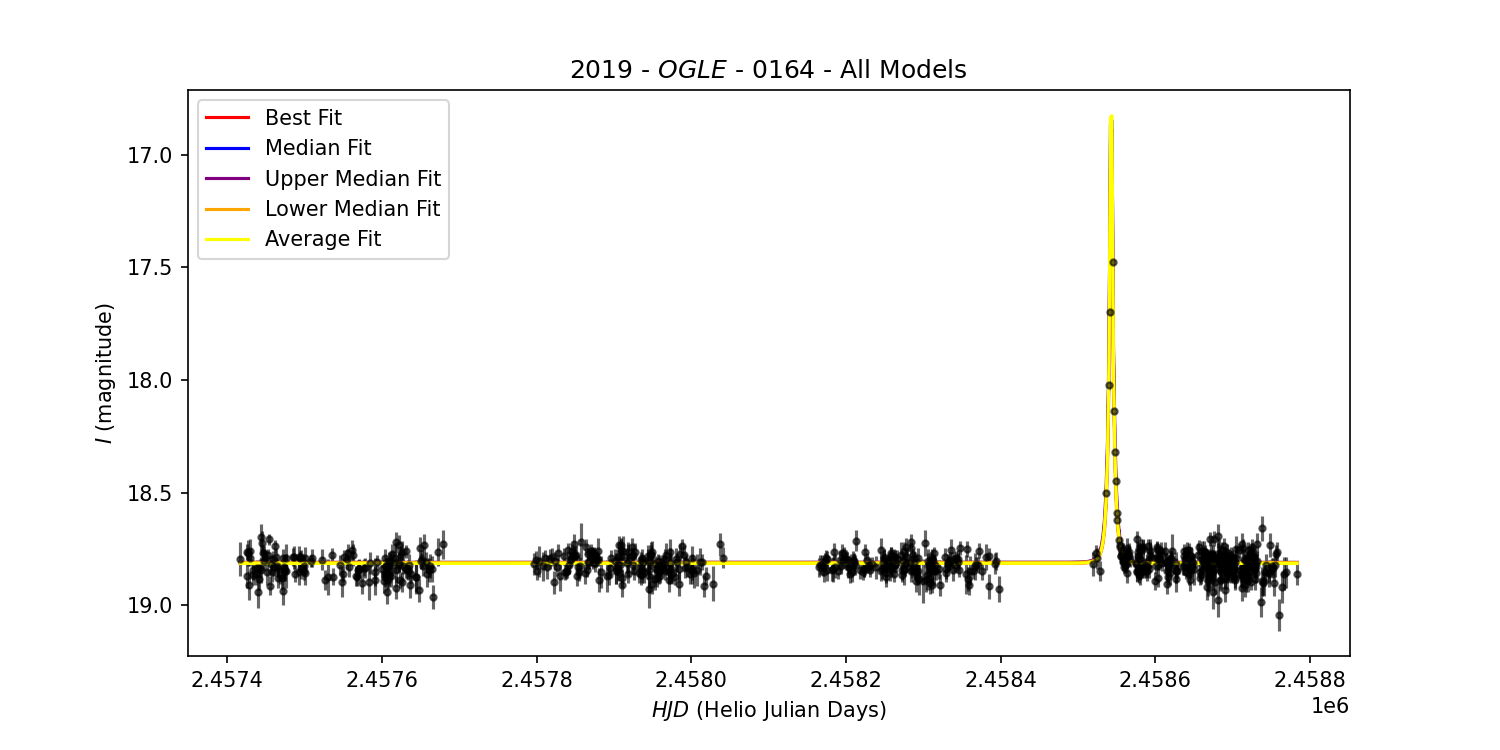
\includegraphics[width=1\linewidth, height=10cm]{Images/2019-BLG-0164_All Models .png}
            \caption{BLG-0164}
            \label{fig:Sub-Event-One-Main}
        \end{figure}

However despite its variability, the models deviate from each other negligibly. For this reason, the other OGLE event data sets were not analyzed through this method. This means that even though there might be many ways of extracting parameters, the optimized ones are ones that fit the best. All other parameters are close enough to them that it is reasonable to ignore them.


\section{Conclusion}
The model fitting of the data sets have revealed critical information about the Paczynski Light Curve. The results from the MCMC analysis shed some light on our inherent biases and assumptions made and how those affect the data. Data Quantification Analysis shows that the model will perform the best when its provided clean data, however it still does relatively well with messy data. There is a direct correlation between the amount of noise and the variability in the parameter. This makes sense because MCMC extracts samples from a given probability distribution. This distribution is ideally the probability distribution of the parameters. It is noteworthy to mention that the conclusions derived from the experiments and the probability distribution of the parameters is based on the initial assumption that all events include point like sources and lenses. This means that  the Paczynski Curve will not necessary be an effective model to predict lensing trajectories for events that aren't single source and lens events, as we cannot make the point-like assumption in those cases.

 \section{Acknowledgements}
 \begin{itemize}
 
\item Aidan Boyce: Helped in initial data set selection. Assisted in getting optimization, the model, and the MCMC graphs. 

\item Yoon Kyu Choi: Helped in initial data set selection and  downloaded OGLE data initially as text files to distribute to everyone in the early stages of the project. Assisted in working with the data files and the optimization. Looked into other sample journals to find one that had similar goals for research and LaTeX and assisted with the model. Pointed out a few possible assumptions and limitations related to this project. Wrote the Introduction and the Data part of the paper.

\item George Kharchilava: Determined how to initially invert y-axis to make the data similar to the one on the OGLE site. Worked with optimization to find the best fit parameters. With Professor Keeton's help, I was able to figure out that the guesses for optimization were the values from the OGLE site and that the best fit parameters then need to be used in the MCMC analysis. Incorporated the residual plots to determine if the models were adequately plotted. With the help of Professor Keeton again, was able to determine which plots we should include in the final code. Finally I created the multiple model plot for the second data set to check how variable the models were when different parameters were used. 

\item Michael Polanco: Helped in initial data set selection from OGLE database. Initially plotted the data points from each data set using the observed time as the x-axis and the magnitude as the y-axis. Collaborated on creating the initial Paczynski model for the analysis and plotting it with the observed data points. Organized the python notebook with Markdown text and helped George with initial residuals plot. Reviewed final paper for grammar adjustments and data/plot information alignment.

\item Geet Purohit: Figured out how to establish a secure FTP connection to the OGLE database to download the \texttt{.phot} data files that are used in the Python Notebook. Since the initial models and incomplete MCMC runs were not efficient nor correct, I wrote the new Paczynski Model, the $\chi^2$ function, the likelihood function and the prior function used for the MCMC analysis, all of which are present in the final notebook. Figured how to run Markov Chain Monte Carlo Simulation using \texttt{emcee} documentation and implemented probability distribution parameters. Worked out and plotted the walkers and the corner plots for all three data sets and made it much more efficient. Helped George perform the Alternative Model Analysis to establish reasonable justification in choosing some data sets over others. Developed the title page for the latex document, and wrote the Methods Section, the Results Section, the Discussion Section, the Conclusion Section, and the References section for the Latex report. Additionally developed the bibliography. Finally, made the entire Microlensing presentation, sourced all the slides and added all the plots and analyses to all the slides.
\end{itemize}

\setlength\bibitemsep{2\itemsep}
\printbibliography
\end{document}
